\documentclass[12pt]{article}

\usepackage{sbc-template}
\usepackage{graphicx,url}
\usepackage[utf8]{inputenc}
\usepackage[T1]{fontenc}
\usepackage[brazil]{babel}
\usepackage{tikz}
\usetikzlibrary{arrows.meta,positioning,shapes.geometric}

\sloppy

\title{Detecção de Imagens Sintéticas após Transformações Digitais}

\author{Nathália G. Ribas\inst{1}, Igor M. da Rosa\inst{1}}

\address{Departamento de Computação (DEC)\\
Universidade Federal de Santa Catarina\\
Araranguá, SC
\email{ribas.nathalia@grad.ufsc.br, igor.matos.rosa@grad.ufsc.br}
}

\begin{document}

\maketitle

\begin{abstract}
This work studies how classical computer vision methods behave when detecting AI-generated images that go through common digital transformations, such as JPEG compression, crop, resize and blur. After reviewing frequency, spatial and texture descriptors (FFT, HOG, LBP) and classifiers (SVM, $k$-NN and CNNs), we adopt an RBF SVM trained on original CIFAKE images and tested on transformed versions, measuring the drop in accuracy for each transformation and each type of feature.
\end{abstract}

\begin{resumo}
Este trabalho estuda como métodos clássicos de visão computacional se comportam ao detectar imagens geradas por IA depois de transformações digitais comuns, como compressão JPEG, crop, resize e blur. Depois de revisar descritores de frequência, espaço e textura (FFT, HOG, LBP) e classificadores (SVM, $k$-NN e CNNs), adotamos um SVM com kernel RBF treinado em imagens originais do CIFAKE e testado nas versões transformadas, medindo a queda de acurácia por transformação e por tipo de feature.
\end{resumo}

%----------------------------------------------------------------------
\section{Introdução}
%----------------------------------------------------------------------

Hoje é fácil gerar imagens realistas com inteligência artificial, o que dificulta saber se uma foto é verdadeira ou criada por um modelo. Em situações práticas --- como posts em redes sociais em período eleitoral ou anúncios de imóveis --- essas imagens quase nunca chegam intactas: passam por compressão, corte, redimensionamento e filtros. Essas mudanças podem enfraquecer os sinais que os detectores usam para reconhecer conteúdo sintético.

A pergunta deste trabalho é: \emph{quão bem detectores baseados em features clássicas continuam funcionando quando a imagem sofre transformações típicas da internet?} Em vez de só classificar ``real versus IA'' em imagens limpas, o foco é um teste de robustez: treinar o classificador com imagens sem transformação e depois medir o quanto o desempenho cai com cada alteração.

Um teste inicial com o site ZeroGPT\footnote{\url{https://www.zerogpt.com/pt/ai-image-detector}} ajuda a ilustrar o problema. Partindo de uma foto real de estúdio, pediu-se a uma IA para mudar a cena (mantendo a pessoa). O ZeroGPT marcou a imagem editada como cerca de 99\% falsa. Depois, apenas comprimindo essa mesma imagem, o resultado passou para cerca de 97\% real --- ou seja, a manipulação deixou de ser detectada (Figura~\ref{fig:zerogpt-editada}).

\begin{figure}[ht]
\centering
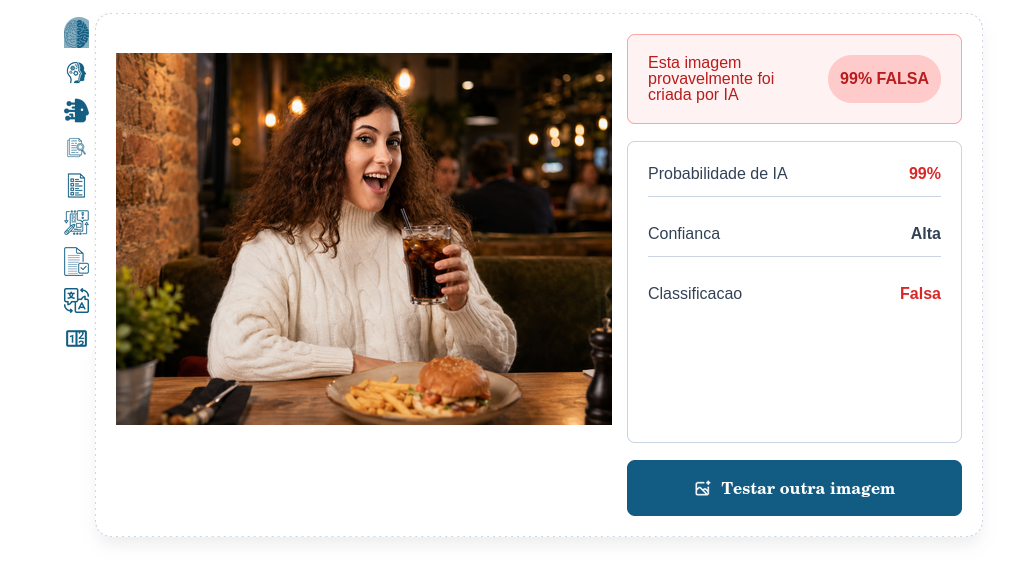
\includegraphics[width=0.48\textwidth]{../Exemplos/EditadaIA/TestePosTransformacao.png}
\hfill
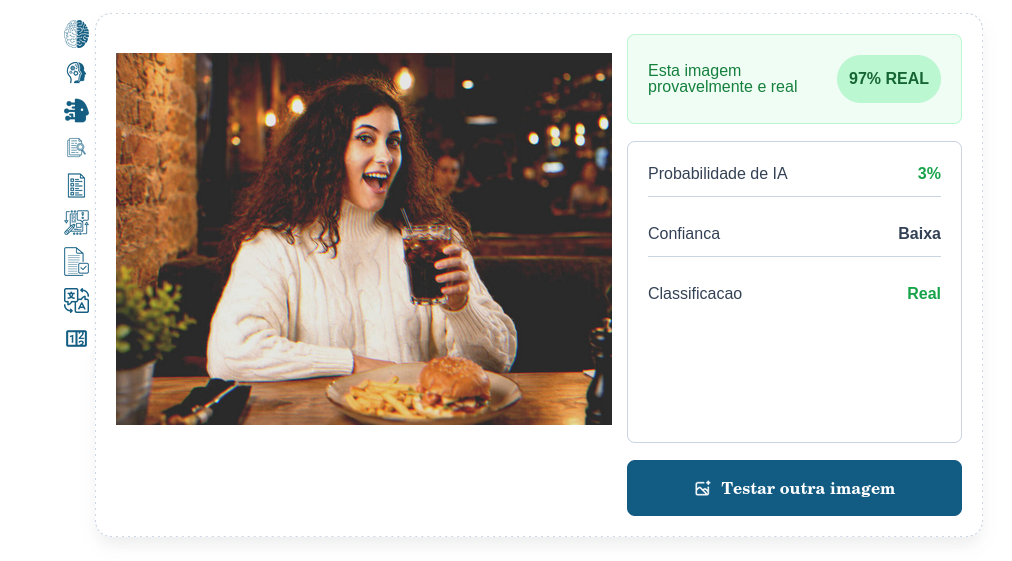
\includegraphics[width=0.48\textwidth]{../Exemplos/EditadaIA/TesteReducaoReso.png}
\caption{Resultados do ZeroGPT. À esquerda: foto real com cena alterada por IA ($\approx$99\% falsa). À direita: a mesma imagem após compressão ($\approx$97\% real), mostrando que o detector falhou.}
\label{fig:zerogpt-editada}
\end{figure}

Este texto complementa o relato anterior. Além do problema e da literatura, passa a descrever as técnicas estudadas (fundamentação teórica) e as escolhas feitas no desenvolvimento: quais features, qual classificador, como o SVM é usado neste problema e quais parâmetros foram fixados no experimento.

%----------------------------------------------------------------------
\section{Trabalhos Relacionados}
%----------------------------------------------------------------------

Vários trabalhos já tratam da detecção de imagens geradas por IA, usando datasets públicos, análise em frequência, features manuais ou redes neurais.

Bird e Lotfi~\cite{bird2024cifake} criaram o CIFAKE, com imagens reais do CIFAR-10 e imagens sintéticas feitas com Stable Diffusion, e obtiveram cerca de 93\% de acurácia com CNN. Esse dataset é a base deste projeto, por ser balanceado, bem documentado e já usado em estudos com features manuais~\cite{nirob2026handcrafted}.

Frank et al.~\cite{frank2020frequency} mostraram que imagens de GANs deixam marcas claras no espectro de frequência, ligadas ao \emph{upsampling}, o que ajuda a separar real de fake e ainda resiste melhor a blur e crop. Bammey~\cite{bammey2024synthbuster} levou essa ideia para modelos de difusão (Synthbuster), olhando picos no espectro de Fourier e conseguindo detectar imagens mesmo com JPEG leve. Por isso faz sentido usar features de frequência e testar compressão JPEG neste trabalho.

Nirob et al.~\cite{nirob2026handcrafted} testaram várias features manuais no CIFAKE (histograma, DCT, HOG, LBP, GLCM, wavelets) com classificadores clássicos e ensembles. A combinação de features teve bom desempenho, o que reforça o uso de FFT, HOG e LBP aqui.

Choi et al.~\cite{choi2025warpad} propuseram o WaRPAD, um método sem treino específico que mede o quanto embeddings mudam com crop/resize. Mesmo sendo uma técnica diferente da nossa, o trabalho mostra que transformações geométricas atrapalham a detecção --- o mesmo tipo de problema que queremos medir.

Em resumo: (i)~frequência e textura ajudam na detecção~\cite{frank2020frequency,bammey2024synthbuster,nirob2026handcrafted}; (ii)~é importante testar transformações realistas~\cite{choi2025warpad,bammey2024synthbuster}. O que este trabalho busca é medir, com features clássicas + SVM no CIFAKE, quanto cada transformação e cada tipo de feature perde desempenho.

%----------------------------------------------------------------------
\section{Fundamentação Teórica}
%----------------------------------------------------------------------

Esta seção descreve as técnicas e os algoritmos estudados para tratar o problema. A justificativa da escolha e o uso no experimento ficam na Seção~\ref{sec:desenvolvimento}.

\subsection{Dois caminhos para detectar imagem sintética}

Há, em linhas gerais, dois jeitos de decidir se uma foto é real ou gerada por IA.

No caminho da \emph{visão clássica}, a imagem é resumida por descritores calculados à mão (frequência, bordas, textura) e um classificador simples --- SVM ou $k$-NN --- aprende a fronteira entre as duas classes~\cite{gonzalez2018,nirob2026handcrafted}. Cada número do vetor tem um significado visual, o que ajuda a explicar por que uma transformação (JPEG, crop, blur) piora o detector.

No caminho do \emph{aprendizado profundo}, uma CNN aprende sozinha quais padrões importam. No CIFAKE, isso chega a cerca de 93\% de acurácia~\cite{bird2024cifake}. O custo é a caixa-preta: fica mais difícil ligar a queda de desempenho a um domínio da disciplina (valor, espaço ou frequência).

Como o problema deste projeto é de \emph{robustez interpretável} --- não só acertar, mas dizer \emph{qual padrão some} após cada transformação --- as duas famílias foram estudadas, mas o foco permanece na via clássica.

\subsection{Domínio da frequência: FFT}

Uma imagem pode ser vista como soma de ondas de diferentes frequências~\cite{gonzalez2018}. A Transformada Rápida de Fourier (FFT) decompõe essa soma. O espectro de magnitude mostra quanto de cada frequência aparece: o centro concentra variações suaves (baixa frequência) e as bordas, detalhes e ruído (alta frequência).

Na detecção de imagens sintéticas, esse domínio importa porque o processo de geração (em especial o \emph{upsampling} de GANs e modelos de difusão) deixa marcas periódicas no espectro~\cite{frank2020frequency,bammey2024synthbuster}. A compressão JPEG também atua em frequência: descarta coeficientes de alta frequência. Por isso a FFT é candidata natural tanto para detectar IA quanto para medir o efeito do JPEG.

Na prática, a FFT 2D da imagem em cinza é deslocada para centralizar as baixas frequências, toma-se o espectro em escala logarítmica e reduz-se o mapa 2D a um vetor 1D (média radial por anéis de frequência). Esse vetor é o descritor usado pelo classificador.

\subsection{Domínio do espaço: HOG}

O Histograma de Gradientes Orientados (HOG) descreve a forma local da imagem~\cite{dalal2005hog}. A ideia é simples: em cada região, mede-se para que lado as bordas apontam (horizontal, vertical, diagonal) e conta-se essas direções num histograma. Juntando os histogramas de várias células, obtém-se um vetor que resume o ``desenho'' da cena, não a cor.

HOG foi proposto originalmente para detecção de pessoas, mas é um descritor espacial padrão e já foi testado no CIFAKE com features manuais~\cite{nirob2026handcrafted}. Recorte e redimensionamento mudam a geometria das bordas; blur as suaviza. Por isso HOG é o descritor natural para observar o efeito de crop, resize e filtros de suavização.

\subsection{Domínio da textura: LBP (e GLCM)}

O Padrão Binário Local (LBP) descreve a textura comparando cada pixel com os vizinhos num círculo~\cite{ojala2002lbp}. Se o vizinho é mais claro, marca 1; se é mais escuro, marca 0. O código binário vira um rótulo do padrão local. O histograma desses rótulos, na versão \emph{uniforme} (invariante a rotação e com poucos bins), é o vetor de features.

A Matriz de Co-ocorrência de Níveis de Cinza (GLCM) é outra forma clássica de textura: conta pares de pixels em certa distância e direção~\cite{gonzalez2018,nirob2026handcrafted}. Também foi estudada, por aparecer no conjunto de features manuais do CIFAKE. LBP é mais barata de calcular e gera um vetor curto, o que importa quando se treina SVM em dezenas de milhares de imagens.

Compressão e blur mudam a relação entre um pixel e seus vizinhos; portanto LBP e GLCM são os descritores em que se espera ver degradação por JPEG forte e por suavização.

\subsection{Classificadores estudados}

Com o vetor de features em mãos, três famílias de classificador foram consideradas.

\paragraph{SVM.}
A Máquina de Vetores de Suporte procura a fronteira que melhor separa as duas classes, maximizando a margem~\cite{cortes1995svm}. Com kernel linear, a fronteira é um hiperplano. Com kernel RBF (\emph{Radial Basis Function}), a fronteira pode ser curva, o que costuma acertar mais quando as classes não são linearmente separáveis. O parâmetro $C$ controla o quanto o modelo insiste em acertar o treino. SVM é o classificador clássico de reconhecimento de padrões da disciplina e funciona bem com vetores de tamanho fixo.

\paragraph{$k$-NN.}
O classificador dos $k$ vizinhos mais próximos atribui à imagem nova o rótulo da maioria dos $k$ exemplos de treino mais próximos~\cite{cover1967knn}. É fácil de explicar, mas a previsão percorre (na forma ingênua) todo o conjunto de treino. Em 100 mil imagens e vetores de centenas de dimensões, isso fica lento. Além disso, $k$-NN sofre se as features não estiverem na mesma escala.

\paragraph{CNN e ensembles.}
Redes convolucionais aprendem filtros e chegam a acurácia alta no CIFAKE~\cite{bird2024cifake}. Ensembles sobre features manuais (por exemplo LightGBM) também foram relatados~\cite{nirob2026handcrafted}. Os dois caminhos foram estudados como referência de desempenho, não como implementação principal: a CNN dificulta ligar o erro a FFT, HOG ou LBP; o ensemble foge do classificador pedido pela especificação clássica da disciplina.

%----------------------------------------------------------------------
\section{Desenvolvimento}
\label{sec:desenvolvimento}
%----------------------------------------------------------------------

Esta seção registra as escolhas feitas depois de estudar as técnicas acima: o que foi adotado, por quê, e como isso se encaixa no problema de robustez após transformações.

\subsection{Justificativa da técnica escolhida}

A combinação adotada é: \textbf{FFT + HOG + LBP}, concatenados (fusão), classificados por um \textbf{SVM com kernel RBF}.

As três features foram escolhidas porque cobrem os três domínios da disciplina e já aparecem na literatura de detecção~\cite{frank2020frequency,bammey2024synthbuster,nirob2026handcrafted,dalal2005hog,ojala2002lbp}. FFT observa marcas de geração e o efeito do JPEG; HOG observa geometria e bordas; LBP observa textura. Isoladas, cada uma responde a um tipo de transformação; juntas, o classificador vê um retrato mais completo da imagem. Nirob et al.~\cite{nirob2026handcrafted} já haviam mostrado que fundir descritores manuais no CIFAKE melhora o resultado --- o que motivou manter a fusão, e não só um descritor.

O SVM foi escolhido em vez de $k$-NN e de CNN por três motivos. Primeiro, é o classificador clássico pedido pela disciplina e tem interpretação clara (fronteira de margem máxima)~\cite{cortes1995svm}. Segundo, com vetor de fusão de 362 dimensões e 100 mil exemplos, $k$-NN fica pesado na predição e depende demais da escala das features. Terceiro, a CNN, embora forte no CIFAKE~\cite{bird2024cifake}, não deixa explícito qual domínio degradou depois do crop ou do JPEG --- exatamente o que o experimento quer medir. Kernel RBF (em vez de SVM linear) foi mantido para seguir a especificação clássica de SVM e porque a separação real/IA nas features manuais não se assume linear.

GLCM, histograma de cor e DCT foram estudados~\cite{nirob2026handcrafted,gonzalez2018}, mas não entram no pipeline principal para não inflar o vetor nem repetir informação já coberta por LBP (textura) e FFT (frequência).

\subsection{Perspectiva de uso no problema}

O problema específico não é só ``esta foto é IA?''. É: \emph{o detector ainda funciona depois que a foto circula na internet?} Por isso o SVM \emph{não} é treinado em imagens transformadas. Ele aprende a fronteira real/IA só nas originais do CIFAKE e, na avaliação, essa fronteira fica congelada. O que muda é o teste: as mesmas imagens passam por JPEG, crop, resize, blur e por um pipeline combinado. A métrica útil é a \emph{queda} de acurácia (baseline menos acerto após a transformação), por feature.

Essa perspectiva liga cada técnica a um sintoma esperado:

\begin{itemize}
\item JPEG altera o espectro $\rightarrow$ deve afetar mais a FFT~\cite{bammey2024synthbuster};
\item crop e resize mudam a geometria $\rightarrow$ devem afetar o HOG~\cite{choi2025warpad,dalal2005hog};
\item blur e compressão forte mudam a vizinhança dos pixels $\rightarrow$ devem afetar o LBP~\cite{ojala2002lbp}.
\end{itemize}

A fusão é a leitura ``completa'' para o detector prático (incluindo um app futuro que devolve a chance de a foto ser IA). FFT, HOG e LBP isolados continuam no experimento justamente para explicar \emph{onde} a robustez quebra.

O fluxo está na Figura~\ref{fig:fluxo}: se a fusão no original for fraca demais, ajustam-se features ou parâmetros e o ciclo se repete. No experimento já executado, a fusão no original alcançou cerca de 92\% de acurácia, o que manteve o desenho (SVM RBF + três descritores) e deslocou o foco para a análise de robustez e para a interface de uso.

\begin{figure}[ht]
\centering
\begin{tikzpicture}[
  node distance=0.55cm and 0.35cm,
  box/.style={draw, rounded corners, align=center, font=\footnotesize,
              inner sep=4pt, minimum width=2.8cm},
  dec/.style={draw, diamond, aspect=2.4, align=center, font=\scriptsize,
              inner sep=1pt},
  arr/.style={-{Latex}, thick}
]
  \node[box, fill=gray!15] (d) {CIFAKE\\real / fake};
  \node[box, below=of d] (f) {Extrair FFT,\\HOG e LBP};
  \node[box, below=of f] (t) {Treinar SVM RBF\\(imagens originais)};
  \node[box, below=of t] (x) {Aplicar\\transformações};
  \node[box, below=of x] (e) {Medir acurácia\\por feature};
  \node[dec, below=0.65cm of e] (q) {Resultado\\aceitável?};
  \node[box, below left=0.75cm and 0.05cm of q, fill=green!12] (ok) {Analisar e\\relatar};
  \node[box, below right=0.75cm and 0.05cm of q, fill=orange!15] (aj) {Ajustar\\features};

  \draw[arr] (d) -- (f);
  \draw[arr] (f) -- (t);
  \draw[arr] (t) -- (x);
  \draw[arr] (x) -- (e);
  \draw[arr] (e) -- (q);
  \draw[arr] (q) -- node[left, font=\scriptsize] {sim} (ok);
  \draw[arr] (q) -- node[right, font=\scriptsize] {não} (aj);
  \draw[arr] (aj.east) -- ++(0.5,0) |- (f.east);
\end{tikzpicture}
\caption{Fluxograma do projeto no CIFAKE: treino com imagens originais, teste após transformações e ajuste se a robustez for baixa.}
\label{fig:fluxo}
\end{figure}

\subsection{Escolhas de implementação}

As decisões abaixo foram fixadas no código (notebook) para deixar o experimento reproduzível e alinhado à fundamentação.

\paragraph{Dados.}
Usa-se o CIFAKE completo~\cite{bird2024cifake}: 100 mil imagens de treino e 20 mil de teste, $32{\times}32$, classes balanceadas (real = CIFAR-10, sintética = Stable Diffusion). Não há coleta própria. Exemplos do ZeroGPT (Figura~\ref{fig:zerogpt-editada}) não entram nas métricas: só motivam o problema. Geradores atuais (ChatGPT, Midjourney etc.) ficam como estudo opcional, sem substituir o CIFAKE.

\paragraph{FFT.}
Imagem em cinza, FFT 2D com deslocamento do espectro, magnitude logarítmica e média radial em 64 faixas. O vetor tem 64 números e é normalizado para $[0,1]$.

\paragraph{HOG.}
Células $8{\times}8$, blocos $2{\times}2$ e 8 orientações --- parâmetros adequados a $32{\times}32$~\cite{dalal2005hog}. O vetor tem 288 números.

\paragraph{LBP.}
Versão uniforme com $P=8$ vizinhos e raio $R=1$, histograma de 10 bins normalizado~\cite{ojala2002lbp}. Foi preferida à GLCM por vetor curto e custo baixo.

\paragraph{Escala e fusão.}
Cada família passa por \texttt{StandardScaler} ajustado \emph{só no treino}, para o SVM não privilegiar a feature de maior magnitude. A fusão concatena os três vetores já escalados, nessa ordem: FFT, HOG, LBP (362 números).

\paragraph{SVM.}
Quatro modelos \texttt{SVC(kernel=rbf, C=10, gamma=scale)}~\cite{cortes1995svm}: um por feature isolada (para comparar domínios) e um na fusão (para maximizar acerto). Grade de $C$ só seria usada em subconjuntos menores; no conjunto completo o $C=10$ fica fixo, porque validação cruzada em 100 mil exemplos com RBF seria inviável no tempo do projeto. Os modelos e os scalers são gravados em arquivos \texttt{.pkl}.

\paragraph{Transformações.}
O catálogo imita circulação digital~\cite{bammey2024synthbuster,choi2025warpad}: JPEG 90/70/50; crop aleatório de 10\%, 25\% e 40\% (com volta a $32{\times}32$); resize para metade e retorno ao tamanho; blur gaussiano $3{\times}3$; pipeline \emph{crop 25\% $\rightarrow$ resize $0{,}5$ $\rightarrow$ JPEG 70}. Depois de cada transformação a imagem permanece RGB $32{\times}32$, para os extratores não mudarem de tamanho.

\paragraph{Avaliação.}
A métrica principal é a acurácia. Compara-se o teste original (baseline) com o teste transformado, por FFT, HOG, LBP e fusão. O classificador não é retreinado. Gráficos de barras e um mapa de calor da queda alimentam a discussão de quais padrões visuais desaparecem.

O próximo passo de uso --- fora do protocolo de medição --- é um aplicativo em Python que carrega o SVM da fusão, recebe uma foto e devolve a probabilidade de ser IA, opcionalmente após as mesmas transformações.

\bibliographystyle{sbc}
\bibliography{referencias-e2}

\end{document}
